\documentclass[a4paper]{article}
 
\usepackage[margin=1in]{geometry}
\usepackage{amsmath,amsthm,amssymb,bbm,wasysym}
\usepackage[czech]{babel}
\usepackage[utf8]{inputenc}
\usepackage[T1]{fontenc}
\usepackage{tikz}
\usepackage{graphicx}
\usepackage{enumitem}
\usepackage{tabto}
\usepackage{amsmath}

\graphicspath{ {./} }

\DeclareMathOperator{\Ex}{\mathbb{E}} % střední hodnota X pomocí $\Ex X$

\newcommand{\N}{\mathbb{N}} % přirozená čísla
\newcommand{\Z}{\mathbb{Z}} % celá čísla
\newcommand{\R}{\mathbb{R}} % reálná čísla

\renewcommand{\qed}{\hfill\blacksquare} % Quod Est Demonstratum (QED) 

% tohle je pro prostředí úkolů
\newenvironment{ukol}[2][]{\begin{trivlist} 
\item[\hskip \labelsep {\bfseries #1}\hskip \labelsep {\bfseries #2}]}{\end{trivlist}}

\linespread{1.15}
 
\begin{document}
 
% --------------------------------------------------------------
%                         Začni ZDE
% --------------------------------------------------------------
 
\title{ Evoluční algoritmy \\ 3. domácí úkol
        } 
\author{Martin Gráf}
\date{4.5.2023}

\maketitle

Úkolem bylo nalézt co nejkratší trasu používající co nejmenší počet vozidel pro zjednodušenou verzi Vehicle Routing Problému pomocí rojového algoritmu. Naše zjednodušení spočívalo v omezení na pouze jeden typ vozidel kterých máme nekonečně mnoho.

\begin{ukol}{Řešení problému}
\begin{itemize}
	\item Jako kostru našeho řešení jsme nestydatě vykradli kód ze cvičení, neboť ho zjevně psala zkušenější ruka a je tak snáz rozšířitelný a přehlednější. Nebyl ovšem připravený na opětovné vracení se do depa, na plnění bodů nákladem, nebo na minimalizaci počtu použitých aut a komplexnější data, museli jsme proto provést následující úpravy:
	\begin{itemize}
		\item Přidání funkce pro čtení dat z xml souborů. Nic komplikovaného, ale výstup této funkce je formátovaný jako seznam tuples Vertex, který je úpravou struktury ze cvičení
		\item Řešiči se předávají extra vstupní parametry s informací o kapacitě použitého auta
		\item Extra grafické funkce pro zobrazování průběhu výpočtu
		\item \textbf{Největší změny} jsme provedli při generování řešení:
		 \begin{itemize}
			\item Každý mravenec začíná v depu
			\item Do depa se vrací pokaždé co vyloží celý svůj náklad (Počet návratů je ekvivalentní počtu použitých aut) + na konci
			\item Nezbývá-li nic doručit, vrací se do depa a ukončuje
			\item Nevrací se do bodů s naplněnou objednávkou
			\item Pravděpodobnost cesty do bodu s naplněnou objednávkou nebo s objednávkou větší než náš náklad je dělena 2
			\item Pravděpodobnost cesty do bodů tyto podmínky nesplňující je násobena 2
			Úpravou těchto pravděpodobností bychom pravděpodobně dosáhli nejlepších zlepšení při další optimalizaci
		\end{itemize}
		\item Fitness funkci jsme mnili překvapivě málo. Na jejím začátku vypočteme minimální počet použitých aut, což závisí na kapacitě aut a součtu objednávek. Každé auto přes tento limit penalizujeme přičtením 100 k fitness, jinak fitness odpovídá ujeté vzdálenosti. 
	\end{itemize}
	\item Použité parametry jsme použili podobné těm na cvičení. Malé datasety nepotřebovaly úpravu. 10 marvenců bylo možná i víc než co bylo třeba k prohledání a je to pouze otázkou dostatečného počtu iterací k nalezení co nejlepšího řešení. 
	\item Mravenců tedy bylo 10 pro 32 i 72 bodů, a 15 pro 422 bodů, abychom prohledali více možných cest mezi velkým množstvím bodů.
	\item Iterací bylo ve všech případech 500
	\item Pro výpočet pravděpodobností feromonů jsme ponechali $\alpha = 1$, $\beta = 3$
\end{itemize}

\end{ukol}

\begin{ukol}{Výsledky}
\begin{itemize}
	\item \begin{center}
		\begin{tabular}{ c c c c }
		  & 32 bodů & 72 bodů & 422 bodů \\ 
		 Využito aut & 5 & 4 & 38\\
		Nejlepší nalezená vzdálenost & 906.9 & 317.9 & 2708.4 \\
		\end{tabular}
	\item Algoritmy byly hotové prakticky hned pro menší datasety, pro velký dataset ovšem trval alespoň tak dlouho, jako trvá udělat jednu horkou čokoládu a část jí vypít. Výpočet přesného časového údaje na základě této informace zanecháme jako cvičení pro čtenáře.
	\item Problém by šel bezpochyby dále optimalizovat, pokud bychom vylepšili úpravy pravděpodobností pro žádoucí/nežádoucí situace. Dále by možná bylo na místě zesílit feromony které po sobě zanechává globální nejlepší řešení.
	\item Závěrem snad jenom zbývá jen poukázat na umělecké sklony našich mravenců, neboť se jim podařilo nakreslit lepší hvězdu než bych zvládl sám.
\end{center}
\end{itemize}
\begin{center}
		\begin{tabular}{ c c c }
		 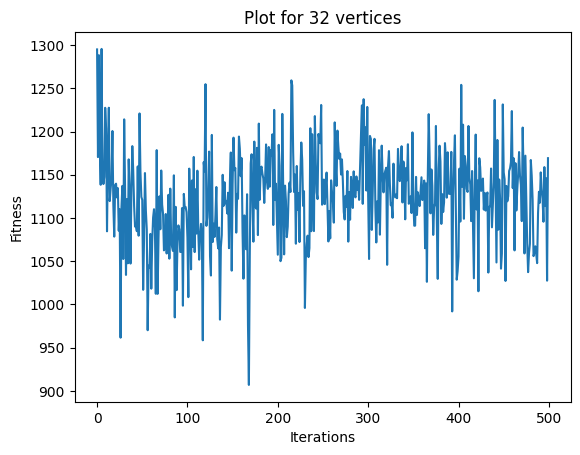
\includegraphics[width=.33\linewidth]{./iterations_32} & 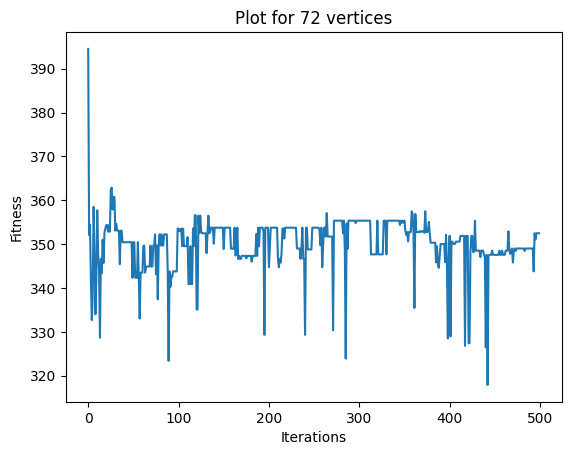
\includegraphics[width=.33\linewidth]{./iterations_72} & 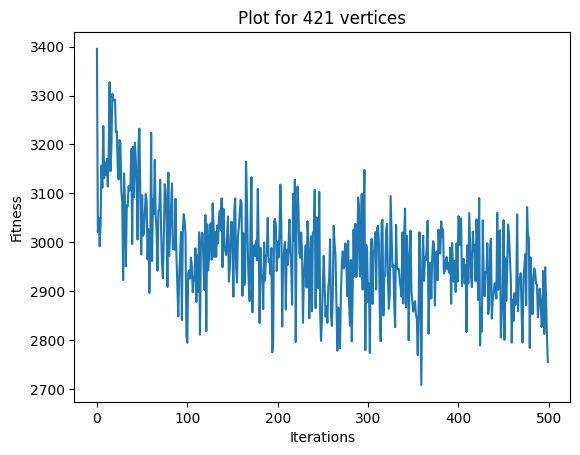
\includegraphics[width=.33\linewidth]{./iterations_422} \\ 
		 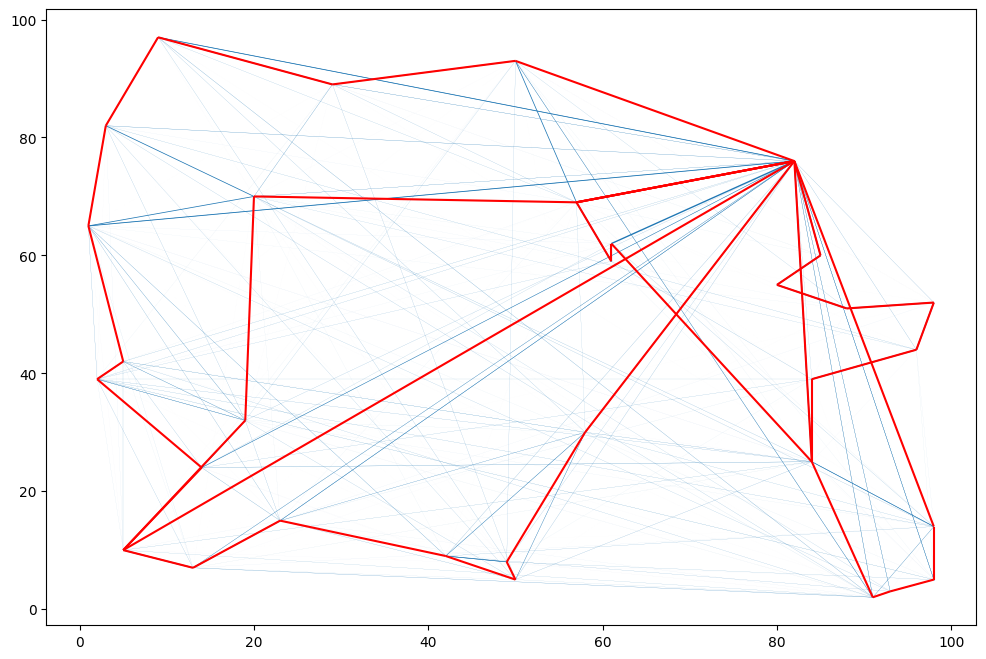
\includegraphics[width=.33\linewidth]{./path_32} & 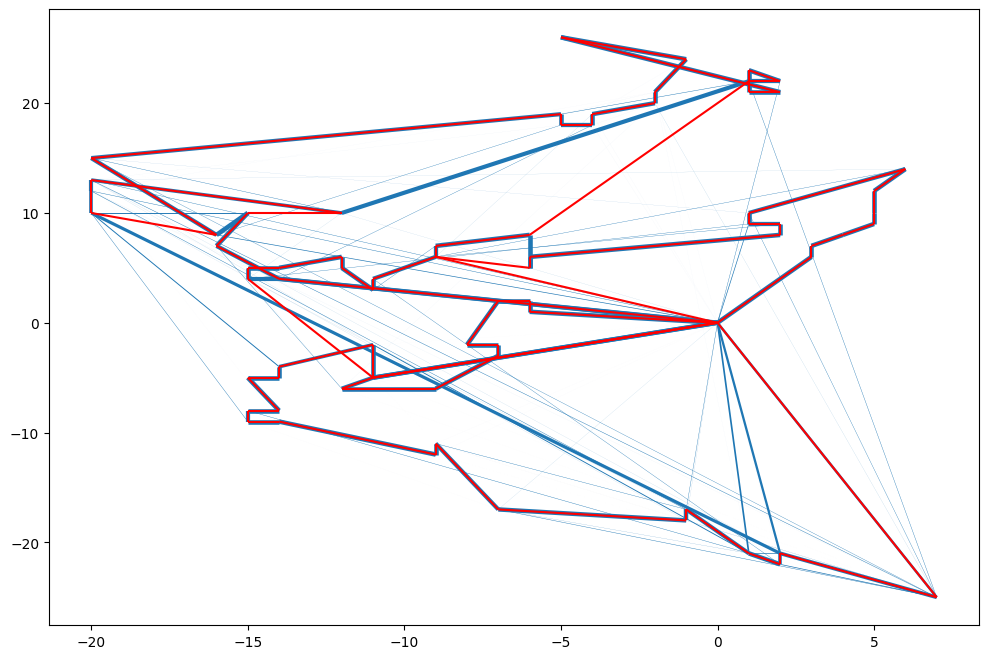
\includegraphics[width=.33\linewidth]{./path_72} & 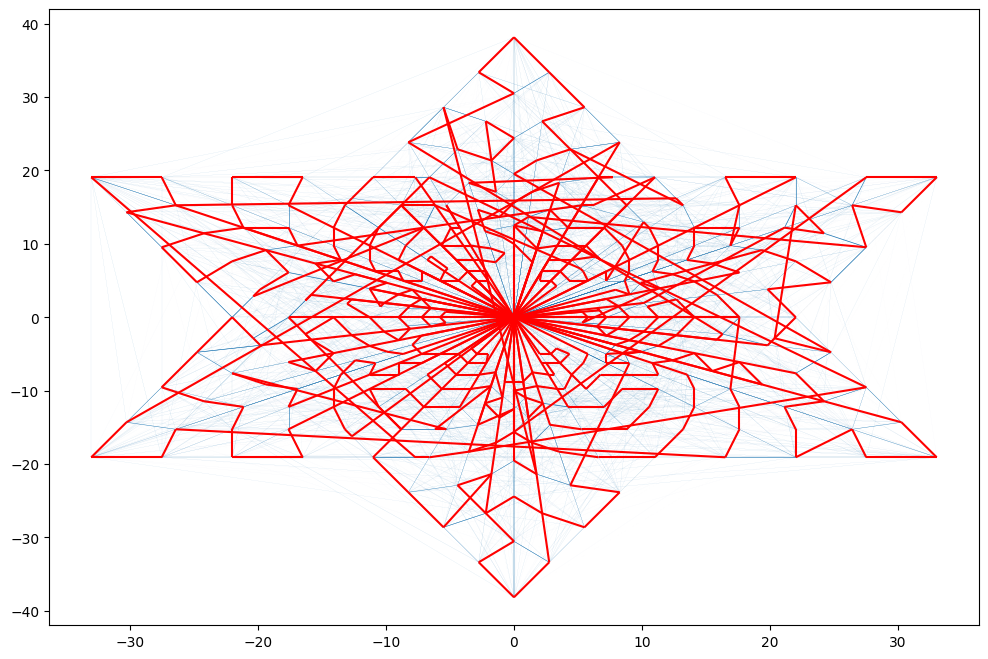
\includegraphics[width=.33\linewidth]{./path_422} \\ 
		\end{tabular}
\end{center}

\end{ukol}

\end{document}
